\documentclass[inci,lof,loc]{imetex}

%% Capa
\author{Igor Cesar Torres de Oliveira}
\title{Análise de Complexidade de Algoritmos Quânticos}
\date{\the\year}

%% Folha de Rosto
\preamble{Relatório Final do Programa Institucional de Bolsas de
Iniciação em Desenvolvimento Tecnológico e Inovação do
CNPq / Instituto Militar de Engenharia.}
\advisor[D.C.]{Prof. Alex Garcia}

%% Resumo
\vernacularAbstract{Usando a computação clássica, baseada em registradores binários e lógica determinística, uma série de problemas computacionais não possuem solução eficiente. Tais problemas são de grande interesse para a humanidade, pois estão relacionados com criptografia, inteligência artificial e problemas NP de modo geral. A computação quântica surge como uma possibilidade para a resolução de tais problemas, principalmente pelos algoritmos quânticos utilizarem processamento simultâneo ao invés de sequencial. Nesse trabalho foram estudados os primeiros algoritmos quânticos de Deutsch, Deutsch-Jozsa, Simon, Grover e Shor, bem como a fundamentação matemática para tal, e implementadas simulações dos algoritmos de Deutsch e Deutsh-Jozsa.}

%% Referências
\references{bibliografia,library}

\begin{document}

\chapter{Introdução}
Na computação clássica o computador é baseado na arquitetura de Von Neumann que faz uma distinção clara entre elementos de processamento e armazenamento de dados, isto é, possui processador e memória destacados por um barramento de comunicação, sendo seu processamento sequencial.
 
Entretanto os computadores atuais possuem limitações, como por exemplo, na área de Criptografia e Segurança de Dados, onde não existem computadores com potência ou velocidade de processamento suficiente para suportar algoritmos de alta complexidade. Dessa forma surgiu a necessidade da criação de um computador diferente dos usuais que resolvesse problemas como a fatoração de números primos muito grandes, logaritmos discretos e simulação de problemas da Física Quântica.
  
Na computação quântica a unidade de informação básica é o bit quântico, também chamado de q-bit ou qubit. Um dos diferenciais da computação baseada em mecânica quântica é que ao invés de assumir valores $0$ ou $1$ de forma determinística como na computação clássica, o qubit pode assumir uma superposição dos estados $\ket{0}$ e $\ket{1}$, colapsando probabilísticamente numa observação.
 
Esta propriedade da superposição de estados que motivou os estudos em computação quântica. Se na computação clássica o processamento é sequencial, na computação quântica o processamento é simultâneo. Através de operadores chamados portas lógicas quânticas, é possivel agir sobre o sistema quântico e com uma única observação obter informações do sistema como um todo.

\section{Justificativa}
A computação quântica é um assunto que está começando a ser estudado na esfera global, embora o computador quântico seja incipiente, já existem alguns algoritmos quânticos, como por exemplo, o algoritmo de Shor para fatoração e algoritmo de Grover para acelerar o processo de procura em banco de dados.
 
Os algoritmos quânticos abrem portas para complexidades inferiores aos já existentes, o que futuramente terá impacto direto em criptografia, inteligência artificial e outras áreas com problemas computacionais difíceis, pois com algoritmos de processamento simultâneo será possível tratar os problemas NP-completos (para os quais não se conhece solução polinomial).

\section{Objetivos}
Este projeto tem como objetivo a análise de caráter geral de algoritmos computacionais quânticos, bem como a comparação com algoritmos da computação tradicional, para resolução de problemas da literatura convencional.

\section{Metodologia}
Foi utilizado o livro Quantum Computing for Computer Scientists para o aprendizado dos capítulos 1, 2, 3, 4, 5 e 6, os quais tratam da base matemática e os algoritmos quânticos introduzidos (capítulo 6).

Utilizando o software ipython notebook e as bibliotecas de uso livre \emph{qutip} e \emph{numpy}, foi implementado um simulador de sistemas quânticos, um simulador da Experiência de Fendas Múltiplas Quântica e implementações dos algoritmos de Deutsch e Deutsch-Jozsa com exemplos resolvidos.

Ao longo do ano foram feitas apresentações após o estudo de cada capítulo do livro, culminando nos simuladores 4.1.1 e 4.5.1 do capítulo 4 do livro, implementados na linguagem de programação python. Findo o estudo do capítulo 6, foi feita a implementação dos algoritmos apresentados.

\section{Cronograma}
O desenvolvimento da pesquisa tem o seguinte planejamento:
\begin{enumerate}
\item Pesquisa bibliográfica do princípio de funcionamento de um computador quântico.
\item Pesquisa sobre as diferenças na programação de algoritmos quânticos em relação à programação binária tradicional.
\item Análise dos algoritmos quânticos específicos.
\item Estudo comparativo dos algoritmos quânticos com os respectivos algoritmos do paradigma tradicional.
\end{enumerate}
Com base nessas atividades, o seguinte cronograma é previsto para o projeto:
\begin{table}[h]
\centering
\begin{tabular}{|c|c|c|c|c|}
\hline 
Atividade & 1º Trimestre & 2º Trimestre & 3º Trimestre & 4º Trimestre \\ 
\hline 
1 & X &   &   &   \\ 
\hline 
2 & X & X &   &   \\ 
\hline 
3 &   & X & X &   \\ 
\hline 
4 &   &   & X & X \\ 
\hline 
\end{tabular}
\caption{Distribuição de atividades}
\end{table}

\chapter{Desenvolvimento}
\section{Simulador de sistemas quânticos}
Os sistemas quânticos são modelados e controlados através de operadores lineares, modelos algébricos das portas lógicas e das dinâmicas dos sistemas. O simulador a seguir implementa um sistema quântico simples, exemplificando como a álgebra matricial determina a distribuição de probabilidades de observação numa medida.
\begin{lstlisting}[language=Python, caption={Simulador quântico básico}, label=simuladorqb]
from numpy import linalg as LA
import numpy as NP

#Matriz de Entrada
M = NP.matrix([[2**(-0.5),2**(-0.5),0],
               [-1j*(2**(-0.5)),1j*(2**(-0.5)),0],
               [0 , 0 , 1j]])

#Estado inicial
X = NP.matrix([[3**(-0.5)],
               [2j*(15**(-0.5))],
               [(2./5)**(0.5)]])

#Numero de clicks
clicks = 1

#Estado apos n clicks
Y = NP.matrix(X)
for i in range (0,clicks):
    Y = M*Y
print Y
\end{lstlisting}

\section{Simulador de Fendas Múltiplas} 
O exemplo a seguir simula o experimento de múltiplas fendas, exemplificando o fenômeno de interferência observado em sistemas quânticos.
\begin{lstlisting}[language=Python, caption={Simulador do experimento de múltiplas fendas}, label=simuladoremf]
from numpy import linalg as LA
import numpy as NP

##################ENTRADAS##################
#Numero de fendas
slits = 2

col = [0]

#Dimensao da matriz
n = 1 + slits + 1 + 2*slits

#Probabilidades de ir para cada slit
p = [2**(-0.5),2**(-0.5)]

############CONSTRUCAO DA MATRIZ############
#Primeira coluna
col = col + p

for k in range (slits+1,n):
    col.append(0)
col = [col]

#Proximas 'slit' colunas
for i in range (0,slits):
    cols = []
    for j in range (0, slits+1+2*i):
        cols.append(0)
    cols.append((-1+1j)/(6**(0.5)))
    cols.append((-1-1j)/(6**(0.5)))
    cols.append((1-1j)/(6**(0.5)))
    k = j+3
    for k in range (k+1,n):
        cols.append(0)
    col = col + [cols]

#Demais colunas
for i in range (slits+1,n):
    cols = []
    for j in range (0, i):
        cols.append(0)
    cols.append(1)
    for k in range (j+2, n):
        cols.append(0)
    col = col + [cols]

#Matriz B
B = NP.matrix(col)
B = B.T

#Entrada inicial X
a = [1]
for i in range (1,n):
    a.append(0)
X = NP.matrix(a)
X = X.T

#Resposta final
Y = NP.matrix((B*B)*X)
print Y

#Interferences
for i in range (slits+1,n):
    if Y[i]==0:
        print "There is an interference in the target " + str(i-slits)
\end{lstlisting}

\section{Algoritmo Deutsch}
O algoritmo de Deutsch é o primeiro exemplo de como o uso de portas quânticas pode reduzir a complexidade de execução de algoritmos. O problema resolvido pelo algoritmo é determinar se uma função $f:\{0,1\}^2\to\{0,1\}$ é balanceada (isto é, $|\{x|f(x)=1\}|=|\{x|f(x)=0\}|$).

Um algoritmo tradicional precisaria fazer duas consultas para observar ambos os valores de $f(x)$, enquanto o algoritmo de Deutsch consegue determinar a resposta para o problema com uma única observação. A estratégia serviu de modelo base para os outros algoritmos quânticos, que operam uma mudança de base no sistema para tirar proveito da superposição de estados. Essa operação é definida na porta lógica $H$, o operador de Hadamard, definido por:
\begin{equation}
\label{eq:hadamard}
\begin{aligned}
H(\ket{0}) = \frac{1}{\sqrt{2}}(\ket{0}+\ket{1}) \\
H(\ket{1}) = \frac{1}{\sqrt{2}}(\ket{0}-\ket{1})
\end{aligned}
\end{equation}


Após a mudança de base, o sistema é sofre a ação do operador $Uf$. Este operador representa a função $f$ numa porta lógica quântica e é assumido como entrada do problema. Seu comportamento é definido por:
\begin{equation}
\label{eq:operatoruf}
Uf(\ket{x}\ket{y}) = \ket{x}\ket{x \oplus f(y)}
\end{equation}


Após a ação de $Uf$, a mudança de base é desfeita e é feita então a observação dos estados dos qubits. Como a observação do primeiro qubit é o suficiente para a solução do problema, o segundo qubit pode ser ignorado após a ação de $Uf$.

Iniciando o sistema no estado $\ket{01}$, O resultado final do sistema será da forma
$$ \pm\frac{1}{\sqrt{2}}\ket{f(0)\oplus f(1)}(\ket{0}-\ket{1}) $$
portanto se a função $f$ for balanceada, observaremos com probabilidade $1$ o primeiro qubit no estado $\ket{1}$, caso contrário observaremos $\ket{0}$.

\begin{figure}[h]
\centering
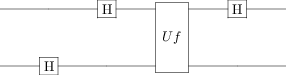
\includegraphics[scale=1]{img/Deutsch.png}
\caption{Diagrama de portas lógicas do algoritmo de Deutsch}
\end{figure}

Na implementação abaixo, instanciamos um circuito lógico (variável \textit{composition}) com o operador identidade e os registradores de qubit no estado inicial $\ket{01}$ (variável \textit{qreg}). Adicionamos então operadores de Hadamard em ambos os qubits através do produto tensorial, criamos operador $Uf$ para uma função $f$ exemplo e adicionamos ao circuito e finalmente adicionamos outro operador Hadamard antes da saída.
\begin{lstlisting}[language=Python, caption={Implementação do algoritmo de Deutsch}, label=deutschimpl]
N = 2 # Numero de fios de entrada
qreg = basis(4,1) # vetor que representa o estado quantico de entrada
circuit = QubitCircuit(N) # instancia um circuito de N fios paralelos
composition = cphase(0) # instancia o circuito com a matriz identidade

H = snot() # instancia uma porta de Hadamard
composition = composition * tensor(H,H) # coloca uma porta de hadamard em cada fio

def U(f): # cria a porta quantica caixa-preta que representa a funcao f
    M = [[(f(0)==0),(f(0)==1),0,0],
         [(f(0)==1),(f(0)==0),0,0],
         [0,0,(f(1)==0),(f(1)==1)],
         [0,0,(f(1)==1),(f(1)==0)]]
    return Qobj(M, dims=[[2,2],[2,2]])

def f(x): # uma funcao exemplo a determinar se e balanceada
    return 1-x

Uf = U(f) # cria a porta quantica da funcao exemplo

composition = Uf * composition # adiciona a porta ao circuito

# adiciona outra porta de hadamard ao circuito para ser lida
composition = tensor(H, rx(0)) * composition

# saida do algoritmo
print qreg.transform(composition)
\end{lstlisting}

No exemplo acima a função $f(x) = 1-x$ leva o estado final a
\begin{lstlisting}
Quantum object: dims = [[4], [1]], shape = [4, 1], type = ket
Qobj data =
[[ 0.        ]
 [ 0.        ]
 [-0.70710678]
 [ 0.70710678]]
\end{lstlisting}
que corresponde ao estado $\frac{1}{\sqrt{2}}\ket{0}(\ket{0}-\ket{1})$. Portanto a observação do primeiro qubit indica função balanceada.

Ao trocarmos a função exemplo para $f(x) = 1$, o estado final será
\begin{lstlisting}
Quantum object: dims = [[4], [1]], shape = [4, 1], type = ket
Qobj data =
[[-0.70710678]
 [ 0.70710678]
 [ 0.        ]
 [ 0.        ]]
\end{lstlisting}
que corresponde ao estado $\frac{1}{\sqrt{2}}\ket{1}(\ket{0}-\ket{1})$. Portanto a observação do primeiro qubit indica função balanceada.

\section{Algoritmo Deutsch-Jozsa}
O algoritmo de Deutsch-Jozsa é uma extensão do algoritmo de Deutsch para funções $f:\{0,1\}^n\to\{0,1\}$, determinando se uma função $f$ (sabido que ela é balanceada ou constante) é balanceada.

O algoritmo demonstra que a diferença no custo de observação do caso base descoberto por Deutsch anteiormente leva a um crescimento exponencial no caso de algoritmos clássicos ao contrário de complexidade constante no caso quântico. Ele serviu de base para os algoritmos de Shor e Grover, que se utilizam de esquemas semelhantes respectivamente para fatorar números e inverter funções.

Enquanto algoritmos clássicos precisam aumentar sua complexidade computacional, algoritmos quânticos aumentam sua complexidade de hardware por se tratar de computação simultânea. O algoritmo de Deutsch-Jozsa aumenta a complexidade de hardware pois precisa de um novo registrador para cada dimensão no espaço de estados quânticos.

\begin{figure}[h]
\centering
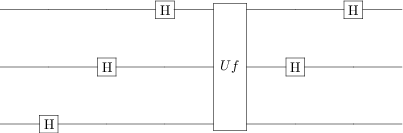
\includegraphics[scale=1]{img/Deutsch-Jozsa.png}
\caption{Diagrama de portas lógicas do algoritmo de Deutsch-Jozsa}
\end{figure}

De forma semelhante ao algoritmo de Deutsch, no sistema final os $n$ primeiros qubits de saída tem uma probabilidade de serem observados no estado $\ket{0}^{\otimes n}$ dada por:
$$ \left| \frac{1}{2^n}\sum_{k=0}^{2^n-1}(-1)^{f(k)} \right|^2 $$
que resulta em $0$ se e somente se $f$ é balanceada e em $1$ se e somente se $f$ é constante.
 
A seguir apresentamos uma implementação para o algoritmo com $n=2$, muito semelhante ao algoritmo de Deutsche (caso $n=1$).  
\begin{lstlisting}[language=Python, caption={Implementação do algoritmo de Deutsch-Jozsa}, label=deutschjozsaimpl]
N = 3
qreg = basis(2**(N),1)
circuit = QubitCircuit(N)
composition = cphase(0,3)

H = snot()
composition = composition * tensor(H,H,H)

def U(f):
    M = [[f(0,0)==0,f(0,0)==1,0,0,0,0,0,0],
         [f(0,0)==1,f(0,0)==0,0,0,0,0,0,0],
         [0,0,f(0,1)==0,f(0,1)==1,0,0,0,0],
         [0,0,f(0,1)==1,f(0,1)==0,0,0,0,0],
         [0,0,0,0,f(1,0)==0,f(1,0)==1,0,0],
         [0,0,0,0,f(1,0)==1,f(1,0)==0,0,0],
         [0,0,0,0,0,0,f(1,1)==0,f(1,1)==1],
         [0,0,0,0,0,0,f(1,1)==1,f(1,1)==0]]
    return Qobj(M, dims=[[2,2,2],[2,2,2]])

def f(x,y):
    return x+y%2

Uf = U(f)

composition = Uf * composition

composition = tensor(H, H, rx(0)) * composition

print qreg.transform(composition)
\end{lstlisting}

O estado final com $f(x,y)=x+y \mod 2 $, por exemplo, é
\begin{lstlisting}
Quantum object: dims = [[8], [1]], shape = [8, 1], type = ket
Qobj data =
[[ 0.        ]
 [ 0.        ]
 [ 0.        ]
 [ 0.        ]
 [ 0.        ]
 [ 0.        ]
 [ 0.70710678]
 [-0.70710678]]
\end{lstlisting}
que representa superposição de estados $\ket{110}$ e $\ket{111}$, logo probabilidade $0$ de observar $\ket{00}$ nos dois primeiros qubits.

Alternativamente para $f(x,y)=1$, temos:
\begin{lstlisting}

Quantum object: dims = [[8], [1]], shape = [8, 1], type = ket
Qobj data =
[[-0.70710678]
 [ 0.70710678]
 [ 0.        ]
 [ 0.        ]
 [ 0.        ]
 [ 0.        ]
 [ 0.        ]
 [ 0.        ]]
\end{lstlisting}
que representa superposição de estados $\ket{000}$ e $\ket{001}$, logo probabilidade $1$ de observar $\ket{00}$ nos dois primeiros qubits.

Podemos ver que a implementação de tais algoritmos usando a computação clássica torna-se muito custosa para casos grandes, pois exige processamento de muitos casos sequencialmente. Porém, se o processamento fosse simultâneo, como aconteceria com um hardware quântico, a complexidade seria na ordem de 1.

\chapter{Conclusão}
Com a implementação dos algoritmos de Deutsch e Deutsch-Jozsa pode-se perceber que tais algoritmos quânticos podem resolver problemas com complexidade muito inferior aos clássicos.

Entretanto todos os casos vistos, a simulação de um computador quântico é mais complexa que o problema original resolvido pelos algoritmos quânticos.

Portanto as simulações são úteis em caráter de prova de conceito e demonstração, porém é necessário a implementação em hardware específico para um real ganho computacional.

\nocite{yanofsky}
\nocite{Guigues}
\end{document}